% vim: set tw=78 sts=2 sw=2 ts=8 aw et:
\documentclass{so.cs.pub.ro}

\usepackage{code/highlight}

\title[Laborator 5]{Laborator 5}
\subtitle{Gestiunea Memoriei}

\begin{document}

\frame{\titlepage}

\begin{frame}{Tipuri de date}
\begin{columns}
\begin{column}[1]{0.55\textwidth}
\framebox{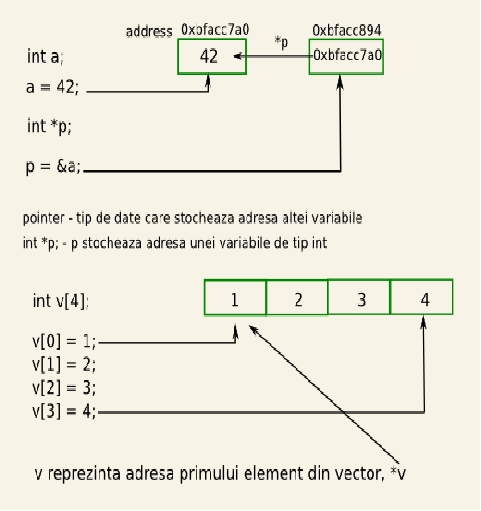
\includegraphics[width=2.2in]{code/tipDate.jpg}}
\end{column}
\begin{column}[1]{0.4\textwidth}
      \begin{itemize}
        \item Primitive (char, int)
        \item Pointer 
        \item Array, Struct 
      \end{itemize}
\end{column}
\end{columns}
\end{frame}

\begin{frame}{Spaţiul de adresă al unui proces}
\framebox{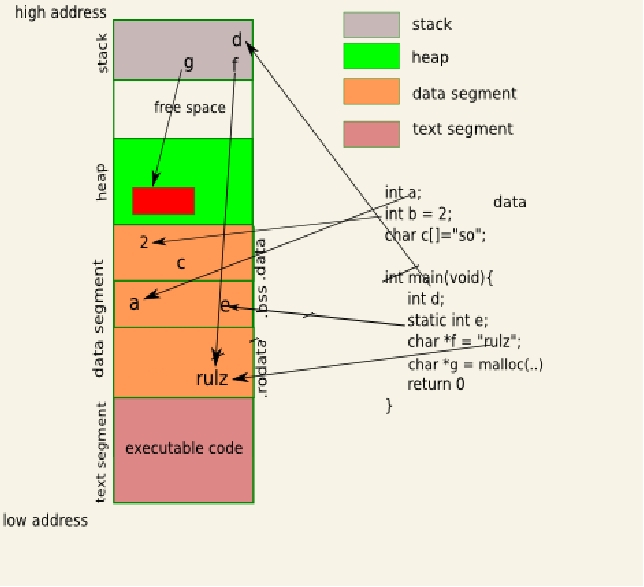
\includegraphics[width=2.5in]{code/spatiuDeAdresa.jpg}}
\end{frame}

\begin{frame}{Pasarea parametrilor pe stivă}
\framebox{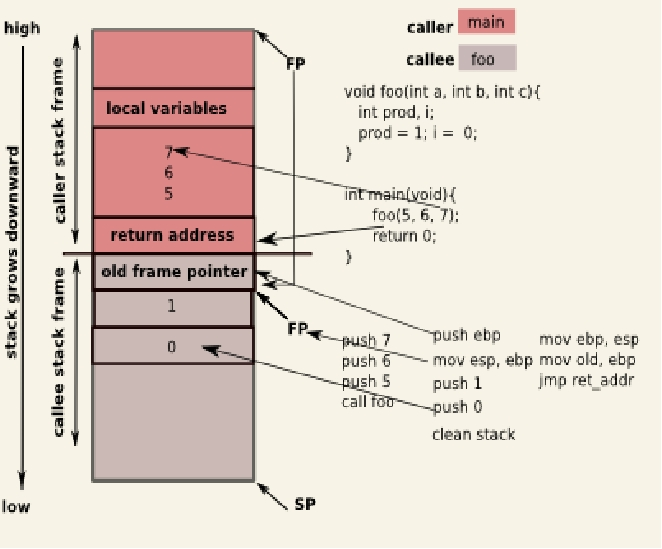
\includegraphics[width=2.5in]{code/passParam.jpg}}
\end{frame}

\begin{frame}{Alocarea memoriei}
  \begin{itemize}
    \item Linux 
    \begin{itemize}
		\item void *malloc(size_t size);
		\item void *calloc(size_t nmemb, size_t size);
		\item void *realloc(void *ptr, size_t size);
		\item void free(void *ptr);    
    \end{itemize}
    \vspace*{0.2cm}
    \item Windows
    \begin{itemize}
		\item HANDLE HeapCreate(flOptions , dwInitialSize, dwMaximumSize);
		\item BOOL HeapDestroy(hHeap);
		\item LPVOID HeapAlloc(hHeap, dwFlags, dwBytes);
		\item HeapReAlloc(hHeap, dwFlags, lpMem, dwBytes);
		\item HeapFree(hHeap, dwFlags, lpMem);   
    \end{itemize}
  \end{itemize}
\end{frame}


\begin{frame}{Probleme de lucru cu memoria}
	\begin{itemize}
		\item acces nevalid
			\begin{beamerboxesrounded}[lower=block body,shadow=true]{}
      		\small{\texttt{char s[4]; sprintf(s,"\%s","so_rulz");}}
			\end{beamerboxesrounded}
		\item memory leak
		\begin{itemize}
		\item pierderea referintei la zona de memorie 
			\begin{beamerboxesrounded}[lower=block body,shadow=true]{}
      		\small{\texttt{for(i = 0; i < 10; i++)\\}}
      		\small{\texttt{\hspace*{0.5in} a = malloc(16*sizeof(int));\\}}
      		\small{\texttt{free(a);}}
			\end{beamerboxesrounded}		
		\end{itemize}
		\item dangling reference
		\begin{itemize}
		\item accesul la o zona de memorie care a fost anterior eliberata 
			\begin{beamerboxesrounded}[lower=block body,shadow=true]{}
      		\small{\texttt{a = malloc(16*sizeof(int));\\}}
      		\small{\texttt{ b = a; free(b);\\}}
      		\small{\texttt{ printf("\%d", a[i]);}}
			\end{beamerboxesrounded}
		\item memoria alocata pentru a a fost eliberata prin intermediul lui b
		\end{itemize}
	\end{itemize}
\end{frame}

\begin{frame}{GDB}
  \begin{itemize}
    \item fișierele trebuie compilate cu opțiunea -g
    \item se transmite ca argument numele executabilului
      \begin{beamerboxesrounded}[lower=block body,shadow=true]{}
        \small{\texttt{gdb ./a.out}}
      \end{beamerboxesrounded}
    \item comenzi GDB utile
      \begin{itemize}
        \item \texttt{bt} - backtrace
        \item \texttt{run} - rulare
        \item \texttt{step, next} - următoarea instrucțiune
        \item \texttt{quit} - părăsirea depanatorului
        \item \texttt{set args} - stabilirea argumentelor de rulare
        \item \texttt{disassamble} - afișează codul mașină generat de compilator
        \item \texttt{info reg} - afișează conținutul registrilor
        \item \texttt{man gdb} - pentru mai multe detalii
      \end{itemize}
  \end{itemize}
\end{frame}

\begin{frame}{mcheck, mtrace}
  \begin{itemize}
    \item mcheck
      \begin{itemize}
			\item verifică consistenţa heap-ului.
			\item MALLOC_CHECK_=1 ./executabil
  		\end{itemize}
        \vspace*{0.4cm}
	 \item mtrace
	   \begin{itemize}
			\item detectează memory leak-urile
			\item mtrace(), muntrace(), pe regiunea inspectată.
  		\end{itemize}
  \end{itemize}
\end{frame}

\begin{frame}{valgrind}
  \begin{itemize}
    \item suită de utilitare pentru debugging şi profiling 
	 \item memcheck, callgrind, helgrind
         \vspace*{0.2cm}
	 \item memcheck 
  \begin{itemize}
	\item valgrind --tool=memcheck ./executabil
	\item detectează
  \begin{itemize}
	\item folosirea de memorie neiniţializată
	\item citire/scriere din/in memorie după ce regiunea respectivă a fost eliberată
	\item memory leak-uri
	\item citirea/scriere dincolo de sfârşitul zonei alocate
	\item folosirea necorespunzatoare a apelurilor malloc/new şi free/delete
	\item citirea/scrierea  pe stivă în zone necorespunzătoare
	  \end{itemize}
	 \end{itemize}
  \end{itemize}
\end{frame}

\begin{frame}{Keywords}
\begin{columns}
\begin{column}[1]{0.55\textwidth}
      \begin{itemize}
        \item Spațiu de adresă
        \begin{itemize}
          \item .text 
          \item .data .rodata .bss
          \item stivă 
          \item heap 
        \end{itemize} 
        \vspace*{0.2cm}             
        \item Alocarea memoriei
        \begin{itemize}
          \item malloc / calloc / realloc 
          \item HeapAlloc / HeapReAlloc
        \end{itemize}
        \vspace*{0.2cm}
        \item Dezalocarea memoriei
        \begin{itemize}
          \item free
          \item HeapFree
        \end{itemize}
      \end{itemize}
\end{column}
\begin{column}[1]{0.35\textwidth}
        \begin{itemize}           
          \vspace*{0.8cm}
          \item accesul nevalid
          \begin{itemize}
          \item gdb
          \item mcheck
          \end{itemize}
          \vspace{0.8cm}
          \item memory leak
          \begin{itemize}
          \item valgrind
          \item mtrace
          \end{itemize}  
          \vspace{1cm}        
        \end{itemize}
\end{column}
\end{columns}
\end{frame}

%\begin{frame}{Întrebări}
%\begin{itemize}
%\item Care este diferența între char a[]="hello" și char *a = "hello";
%\item Cum ați implementa o funcție care aloca N octeți pe stivă? Cum arată funcția free în acest caz?
%\item Cum putem determina direcția de creștere a stivei? (de la adrese mari la adrese mici sau invers)
%\end{itemize}
%\end{frame}


\end{document}
